\documentclass{article}
\PassOptionsToPackage{numbers,square,sort&compress}{natbib}
% Official style, copied without modifications. Named working version.
% Confirm the workshop's anonymity policy before submission.
\usepackage[sglblindworkshop]{neurips_2026}
\workshoptitle{The 2nd Workshop on Embodied Spatial Reasoning}
\usepackage[utf8]{inputenc}
\usepackage[T1]{fontenc}
\usepackage{amsmath,amssymb,amsfonts,amsthm,booktabs,graphicx,microtype,xcolor}
\usepackage{tikz}
\usetikzlibrary{arrows.meta,positioning}
\usepackage{hyperref,url}
\hypersetup{colorlinks=true,linkcolor=teal!65!black,citecolor=teal!65!black,urlcolor=teal!65!black}
\newtheorem{proposition}{Proposition}
\newcommand{\TaskN}{480}
\newcommand{\FamilyN}{120}
\newcommand{\SensorTrainN}{12000}
\newcommand{\SensorTestN}{4000}
\newcommand{\SensorAccuracy}{91.62}
\newcommand{\SensorBrier}{0.0628}
\newcommand{\BeforeSteps}{39}
\newcommand{\AfterSteps}{23}
\newcommand{\LongestReplayMs}{12.62}
\newcommand{\LongestIndexedMs}{0.56}
\newcommand{\LongestExplicitMs}{0.45}

\title{Retractable Imagination:\\Evidence-Addressable Spatial Prediction for Interactive Replanning}
\author{Vaibhav Kanojia\\[3pt]\href{https://github.com/VaibhavKanojia3773/retractable-imagination}{\scriptsize\texttt{github.com/VaibhavKanojia3773/retractable-imagination}}}
\begin{document}
\maketitle
\begin{abstract}
An embodied agent may correct its spatial map yet continue to act on an imagined future derived from invalid evidence. We present Retractable Imagination, a system that connects evidence-addressable inference, forecast invalidation, and replanning while preserving actions already executed. A learned observation encoder supplies occupancy scores; an indexed ledger supports exact removal under a static, factorized model. On \TaskN{} seeded navigation episodes from four controlled task families, corrected states agree with history replay within $4.45\times10^{-16}$ log-odds and unaffected factors remain unchanged. Correction resolves the invalid-passage failures in both false-free-space families. In false-obstacle episodes, it reduces median remaining route length from \BeforeSteps{} to \AfterSteps{} steps, an improvement hidden by success rate alone. With 32,768 encoded observations, backend revision, forecasting, and planning take a median \LongestIndexedMs{}\,ms versus \LongestReplayMs{}\,ms for replay. Explicit sufficient-statistic inference achieves equivalent corrected decisions and comparable latency. The contribution is an inspectable execution contract: retract identified evidence, repair its dependent predictions, and act from the current physical state. The released code includes the interactive artifact, measured data, and reproducible paper sources.
\end{abstract}

\section{Introduction}
A mobile agent has already moved toward a passage when a camera report is declared invalid. The passage did not change; the evidence was wrong. The agent must revise what it believes about the current scene, reconsider futures based on that belief, and act from the position it actually reached. Replacing an observation with a correction does not establish that every downstream inference has been repaired.

Spatial agents must construct and revise beliefs~\cite{zhang2026theory}, and structured memory supports long-horizon decisions~\cite{cherepanov2026elmur}. We test correction as an execution contract: forecasts should match inference on a corrected history, independent predictions should remain stable, and realized actions must remain part of the episode. The target is episode-state inference, not training-data unlearning.

We implement this contract in a compact spatial prediction and planning system. Its three inspectable properties are \emph{correction}, agreement with corrected-history inference; \emph{retention}, stability of independent predictions; and \emph{action continuity}, preservation of the realized episode. The implementation combines a learned observation encoder with additive sufficient statistics, making an exact replay reference available. Evaluation separates repairing an unsafe route, removing an unnecessary detour, and retaining valid state. The contribution is this integrated demonstrator and protocol, rather than a new Bayesian update.

\begin{figure}[t]
\centering
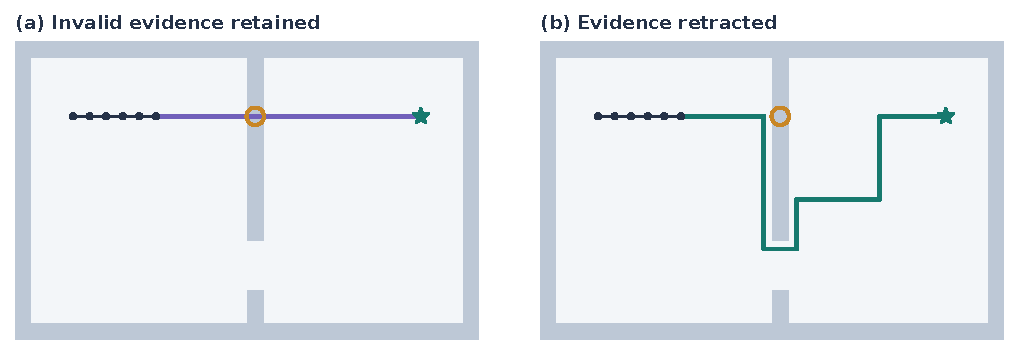
\includegraphics[width=\linewidth]{figures/retraction_scene.pdf}
\caption{\textbf{Revise the belief, preserve the episode.} The original forecast crosses a physically blocked passage after an invalid free-space report. Retracting that report changes the route from the current position. The five-action prefix (dark dots), physical obstacle (amber circle), and goal (star) are unchanged. Routes are computed by the implemented planner; the truth map is shown only for illustration.}
\label{fig:scene}
\end{figure}

\section{Our evidence-addressable system}
Let $H_t$ contain observations and the actions actually executed up to time $t$. When observation identifiers $R$ are revoked, the reference history $H_t^{-R}$ omits those observations but retains the executed actions, subsequent valid evidence, and timestamps. Agreement with inference on $H_t^{-R}$ is an internal consistency target, not a guarantee that the model describes the true physical world.

\paragraph{Learned observation scores.}
Each packet $e$ records an identifier, source, timestamp, cell $c(e)$, and detector features. A logistic model maps a signed sensor response $r$ and quality $q$ to
\begin{equation}
d_\theta(e)=\operatorname{clip}\!\left(\theta^\top[r,rq,q,1],-8,8\right).
\end{equation}
The model uses balanced synthetic occupied/free training examples. Its logit acts as a likelihood-ratio score subject to calibration; inputs are simulated detector features, not raw images.

\paragraph{Indexed predictive state.}
For binary cell occupancy $m_c$, a fixed prior log-odds $L_0(c)$, and active evidence $A$, the state is
\begin{equation}
L_A(c)=L_0(c)+\sum_{e\in A:\,c(e)=c}d_\theta(e),
\qquad p_A(c)=\sigma(L_A(c)).
\label{eq:state}
\end{equation}
An immutable ledger retains the contribution of every packet. Revocation subtracts each active contribution once and marks its record inactive. Repeated revocation is idempotent; an unknown identifier is rejected before mutation.

\begin{proposition}[Restricted replay consistency]
For a fixed prior and immutable additive observation scores, subtracting contributions indexed by $R$ gives $L_{A\setminus R}$, up to floating-point summation order.
\end{proposition}
\begin{proof}
Partition Equation~\ref{eq:state} over $A\setminus R$ and $A\cap R$; subtraction cancels the latter terms.
\end{proof}
This is the standard sufficient-statistic identity underlying the implementation, not a new theoretical result. It does not extend automatically to correlated likelihoods, joint calibration, temporal smoothing, or arbitrary recurrent compression.

\begin{figure}[t]
\centering
\resizebox{\linewidth}{!}{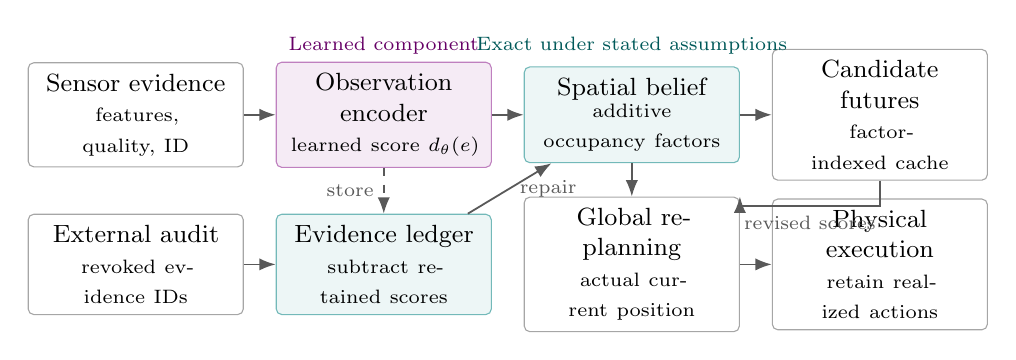
\begin{tikzpicture}[
  >=Latex,
  block/.style={draw=black!35, rounded corners=2pt, align=center, minimum height=1.0cm, text width=2.45cm, inner sep=4pt, font=\small},
  learned/.style={block, fill=violet!8, draw=violet!50},
  analytic/.style={block, fill=teal!7, draw=teal!55},
  link/.style={->,line width=.65pt,draw=black!65},
  note/.style={font=\scriptsize,text=black!65,align=center}
]
\node[block] (obs) at (0,0) {Sensor evidence\\\scriptsize features, quality, ID};
\node[learned] (encoder) at (3.15,0) {Observation encoder\\\scriptsize learned score $d_\theta(e)$};
\node[analytic] (belief) at (6.3,0) {Spatial belief\\\scriptsize additive\\occupancy factors};
\node[block] (cache) at (9.45,0) {Candidate futures\\\scriptsize factor-indexed cache};
\node[block] (audit) at (0,-1.9) {External audit\\\scriptsize revoked evidence IDs};
\node[analytic] (ledger) at (3.15,-1.9) {Evidence ledger\\\scriptsize subtract retained scores};
\node[block] (planner) at (6.3,-1.9) {Global replanning\\\scriptsize actual current position};
\node[block] (execute) at (9.45,-1.9) {Physical execution\\\scriptsize retain realized actions};
\draw[link] (obs)--(encoder);
\draw[link] (encoder)--(belief);
\draw[link] (belief)--(cache);
\draw[link] (audit)--(ledger);
\draw[link] (ledger)--node[note,right]{repair}(belief);
\draw[link] (belief)--(planner);
\draw[link] (cache.south)--++(0,-.32)-|node[note,near start,below]{revised scores}(planner.north east);
\draw[link] (planner)--(execute);
\draw[link,dashed] (encoder)--node[note,left]{store}(ledger);
\node[note,text=violet!80!black] at (3.15,.88) {Learned component};
\node[note,text=teal!70!black] at (6.3,.88) {Exact under stated assumptions};
\end{tikzpicture}
}
\caption{\textbf{System architecture.} Only the observation encoder is learned. The ledger repairs additive spatial factors; affected fixed-route forecasts are invalidated before the planner selects a new action. Replanning uses the actual current position. The audit supplies revocation identifiers externally.}
\label{fig:architecture}
\end{figure}

\paragraph{Forecast dependencies and action selection.}
For a fixed route $\pi$, the model predicts
\begin{equation}
\widehat{P}(\text{no occupied cell}\mid\pi,A)=\prod_{c\in\pi}(1-p_A(c)),
\label{eq:forecast}
\end{equation}
under independent static occupancy. A reverse index links spatial factors to cached route forecasts. When a factor changes, forecasts depending on it are invalidated. Candidates with unchanged factors retain their values. This locality statement applies to a \emph{fixed forecast}: finding the preferred route can depend on the entire map, so route selection is rerun globally.

Risk-aware A* blocks cells with $p_A(c)\geq0.55$ and uses transition cost $1+3[-\log(1-p_A(c))]$ elsewhere. Ground-truth occupancy is used only to score routes and prevent simulated collisions. Actions and the realized trajectory are never rolled back by editing evidence. Figure~\ref{fig:architecture} separates learned encoding, exact correction, and execution.

\section{Implementation and demonstration artifact}
The released implementation exposes a spatial scene, an evidence ledger, and candidate action forecasts through a self-contained interactive artifact. Its code supports packet inspection and revocation, state-consistency checks, dependency-aware forecast invalidation, and stepwise or automatic agent execution. The artifact keeps the original route and realized action prefix visible alongside the revised plan. Ground truth is available only as a labeled evaluation overlay.

The repository includes matching Python and JavaScript inference, evaluation code, measured data, and a standalone HTML entry point. Isometric and top-down views render live predictions on the same two-dimensional state, not validated three-dimensional dynamics. The executable artifact links correction to observable agent behavior and limitations~\cite{esr2026demo}.

\section{Evaluation}
We evaluate three properties separately: replay consistency of the spatial state, retention and invalidation of fixed-route forecasts, and consequences for executed actions. The observation encoder and planner are frozen across all methods. Raw episode records, seeds, timing samples, and the code generating tables are included with the artifact.

\paragraph{Sensor model.}
The encoder is fitted with 180 gradient steps on \SensorTrainN{} synthetic examples and evaluated on \SensorTestN{} separately sampled examples. Held-out accuracy is \SensorAccuracy\,\% and Brier score is \SensorBrier{}. These results characterize the synthetic detector distribution, not real visual perception.

\paragraph{Spatial task protocol.}
Four predeclared samplers generate \FamilyN{} episodes each: false free space, a false obstacle, a revoked source packet group, and a no-corruption control. Room dimensions, partition and passage coordinates, prior strengths, background measurements, and corrupt sensor responses vary by episode. A structural map and informative passage priors are supplied: the experiment isolates correction of injected faulty evidence, not discovery of unknown geometry. Audits follow up to five safe actions from the original plan; their realized prefix is preserved. The no-corruption control supplies an empty audit.

\paragraph{Comparators.}
Full replay reconstructs state from non-revoked evidence. Checkpoint replay starts from the last checkpoint preceding the earliest revoked packet. Explicit subtraction updates the additive state directly. Indexed retraction additionally resolves identifiers through the ledger. A stale-belief control performs no correction. A stale-cache ablation repairs state but continues to use its previous planned route, isolating the consequence of failing to invalidate a derived forecast. This ablation is an intentionally incomplete system, not a competitive inference baseline.

\begin{table}[t]
\centering\small
\begin{tabular}{lrrrr}
\toprule
Task family & Stale & Stale cache & Replay & \textbf{Ours} \\
\midrule
False free space & 0/120 & 0/120 & 120/120 & 120/120 \\
False obstacle & 120/120 & 120/120 & 120/120 & 120/120 \\
Source packet group & 0/120 & 0/120 & 120/120 & 120/120 \\
No corruption & 120/120 & 120/120 & 120/120 & 120/120 \\
\bottomrule
\end{tabular}
\vspace{7pt}
\caption{\textbf{Successful routes on the controlled task distribution.} Ours is evidence-indexed retraction with forecast invalidation and replanning. Each family has \FamilyN{} episodes. The stale-cache ablation retains the old route after state repair. Checkpoint replay and explicit subtraction match replay and ours exactly; no superiority among exact methods is implied.}
\label{tab:tasks}
\end{table}

\paragraph{State consistency and retention.}
Across \TaskN{} task episodes, the maximum absolute discrepancy between indexed state correction and corrected-history replay is $4.45\times10^{-16}$ log-odds. Factors not indexed by revoked packets have zero measured drift. A separate controlled cache test uses 64 disjoint candidate routes: one forecast is invalidated, 63 are retained, and both maximum forecast discrepancy and unaffected-route drift are zero. An explicit implementation with the same dependency index has the same property; this test does not establish that dependencies will be sparse in a coupled world model.

\paragraph{Action consequences.}
Table~\ref{tab:tasks} separates unsafe false-free-space reports from false obstacles. In the latter family, every method reaches the goal, but correction reduces median remaining path length from \BeforeSteps{} to \AfterSteps{} grid steps. Thus success alone misses a practical cost of stale evidence. The empty-audit control produces no state change. These results apply to the specified passage-task samplers; they do not estimate unrestricted navigation success. For 120/120 successes, the Wilson 95\,\% interval is approximately $[96.9\%,100\%]$ within the sampler, not across real deployments.

\begin{figure}[t]
\centering
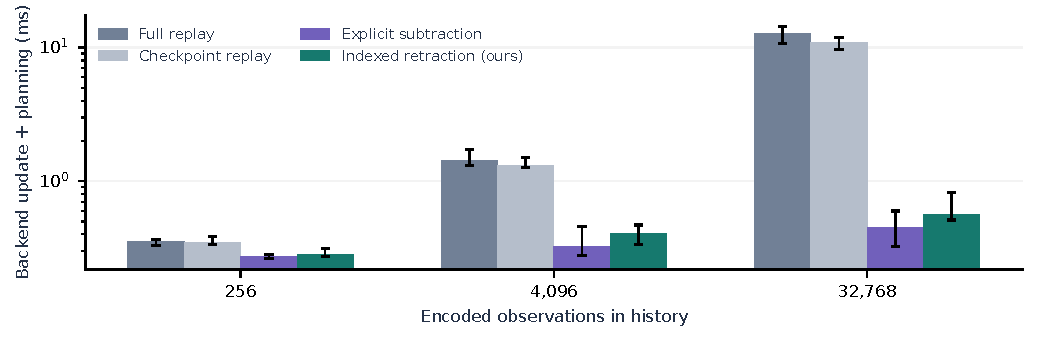
\includegraphics[width=\linewidth]{figures/backend_latency.pdf}
\caption{\textbf{Backend latency with shared downstream work.} Revision, 20 route forecasts, and global A* are timed together. Bars show medians and whiskers show interquartile ranges over 24 independent histories per length; method order is randomized. Acquisition, encoding, initial ingestion, browser rendering, and network time are excluded. The vertical axis is logarithmic.}
\label{fig:latency}
\end{figure}

\paragraph{Computation.}
Figure~\ref{fig:latency} reports backend latency for histories of 256, 4,096, and 32,768 pre-encoded observations, with a revocation at 10\,\% of history. At the longest history, full replay takes a median \LongestReplayMs{}\,ms, indexed retraction \LongestIndexedMs{}\,ms, and explicit subtraction \LongestExplicitMs{}\,ms. All methods recompute the same 20 forecasts and global plan in this test. Indexed and explicit updates implement the same algebra; their differences do not support a claim of algorithmic superiority. Initial indexing, checkpoint construction, and metadata storage are additional costs. Numeric-array memory figures in the raw kernel experiment exclude Python bookkeeping and should not be interpreted as total memory consumption.

\section{Discussion and limitations}
Evidence retraction must be judged at the level where the agent uses it: revised spatial factors, coherent candidate futures, and actions from the current state. The demonstration makes a stale derived forecast observable even when the underlying map has already been repaired. It also exposes the classical control: explicit inference performs the same correction.

The contract assumes static independent factors, immutable scores, and externally supplied revocation IDs. Removing a source group does not model its statistical correlation. Automatic fault detection, coupled calibration/smoothing, and arbitrary recurrent-state correction are not evaluated. Supplied structural maps and simulated detector features restrict the claims to controlled spatial inference and planning, without real-robot or image-model validation.

Incremental smoothing already exploits structured dependencies for efficient inference~\cite{kaess2012isam2}. Contextual belief management also separates updating, retaining, and isolating evidence in synthetic reasoning tasks~\cite{xu2026cbm}. Our artifact connects this distinction to spatial forecasts and executed actions. Extending its contract to learned non-additive state requires comparison with coupled explicit inference and tuned replay; the current results do not resolve that research question.

\bibliographystyle{plainnat}
\bibliography{references}

\appendix
\section{Reproduction and measurement details}
Seeds are 20261102 (tasks), 20261103 (backend timing), and 20261101 (sensor fitting). The repository documents exact evaluation, test, figure-generation, and paper-build commands; measured snapshots are included.

\begin{center}
\begin{minipage}{\linewidth}
\makeatletter\def\@captype{table}\makeatother
\centering\small
\begin{tabular}{lrrrr}
\toprule
History & Replay & Checkpoint & Explicit & \textbf{Ours} \\
\midrule
256 & 0.352 & 0.347 & 0.273 & 0.284 \\
4,096 & 1.427 & 1.310 & 0.325 & 0.409 \\
32,768 & 12.621 & 10.949 & 0.448 & 0.560 \\
\bottomrule
\end{tabular}
\vspace{7pt}
\caption{\textbf{Backend medians in milliseconds}, corresponding to Figure~\ref{fig:latency}. Ours denotes evidence-indexed retraction. All timings include revision, 20 forecasts, and global planning. Full samples and interquartile ranges are in \texttt{data/study.json}.}
\end{minipage}
\end{center}

\end{document}
